\documentclass[aspectratio=43,10pt]{beamer}

% Theme & Styling
\usetheme{Madrid}
\usecolortheme{whale}

% -----------------------------------------------------------------------------
% Elegant Obsidian / Dark Aesthetic Palette (Grant Sanderson 3Blue1Brown Style)
% -----------------------------------------------------------------------------
\definecolor{DarkCanvas}{RGB}{12, 16, 24}      % Deep obsidian canvas
\definecolor{DarkBox}{RGB}{20, 27, 40}         % Translucent dark card
\definecolor{DarkBoxInner}{RGB}{26, 36, 54}    % Accent box background
\definecolor{LuminousGold}{RGB}{245, 190, 60}  % Vibrant Gold / ITB Gold
\definecolor{ElectricBlue}{RGB}{80, 165, 250}  % Luminous Sky Blue
\definecolor{TealCyan}{RGB}{45, 212, 191}      % Cyan / Teal
\definecolor{EmeraldGreen}{RGB}{52, 211, 153}  % High-contrast green (Maks/Min)
\definecolor{CoralRose}{RGB}{251, 113, 133}    % High-contrast rose (Peringatan/Ekstrem)
\definecolor{PurpleBelok}{RGB}{216, 140, 255}  % Vivid lilac
\definecolor{SoftGray}{RGB}{200, 210, 225}     % Readable muted text

% Apply Dark Colors to Beamer Elements
\setbeamercolor{background canvas}{bg=DarkCanvas}
\setbeamercolor{normal text}{fg=white}
\setbeamercolor{structure}{fg=ElectricBlue}
\setbeamercolor{title}{fg=white,bg=DarkBox}
\setbeamercolor{frametitle}{fg=LuminousGold,bg=DarkBox}
\setbeamercolor{footline}{fg=SoftGray!70,bg=DarkCanvas}
\setbeamercolor{headline}{fg=SoftGray!70,bg=DarkCanvas}

% Block Styles in Dark Theme
\setbeamercolor{block title}{fg=white,bg=ElectricBlue!45!black}
\setbeamercolor{block body}{fg=white,bg=DarkBox}
\setbeamercolor{block title example}{fg=white,bg=EmeraldGreen!40!black}
\setbeamercolor{block body example}{fg=white,bg=DarkBox}
\setbeamercolor{block title alerted}{fg=white,bg=CoralRose!45!black}
\setbeamercolor{block body alerted}{fg=white,bg=DarkBox}

% Lists & Numbering
\setbeamercolor{item}{fg=LuminousGold}
\setbeamercolor{subitem}{fg=TealCyan}
\setbeamercolor{enumerate item}{fg=LuminousGold}
\setbeamercolor{enumerate subitem}{fg=TealCyan}

% Packages
\usepackage[utf8]{inputenc}
\usepackage{amsmath,amssymb}
\usepackage{graphicx}
\usepackage{hyperref}
\usepackage{multimedia}
\usepackage{tikz}

\hypersetup{
    colorlinks=true,
    linkcolor=TealCyan,
    urlcolor=ElectricBlue
}

\title[MA1101 Matematika I]{MA1101 Matematika I --- Bab 3: Penggunaan Turunan}
\subtitle{Subtopik 3.3: Ekstrem Lokal dan Ekstrem pada Selang Buka\\(\textit{Local Extrema and Extrema on Open Intervals})}
\author[FMIPA ITB]{Tim Pengajar MA1101}
\institute[ITB]{Fakultas Matematika dan Ilmu Pengetahuan Alam\\Institut Teknologi Bandung}
\date{Semester 1 Tahun Akademik 2026/2027}

\begin{document}

% -------------------------------------------------------------
% Slide 1: Judul
% -------------------------------------------------------------
\begin{frame}
    \titlepage
\end{frame}

% -------------------------------------------------------------
% Slide 2: Motivasi & Tantangan Sokratik (The Pique)
% -------------------------------------------------------------
\begin{frame}{Tantangan Awal: Optimasi Tanpa Dinding Batas}
    \begin{columns}[T]
        \begin{column}{0.55\textwidth}
            \begin{block}{Dilema Tanpa Batas $[a, b]$}
                \begin{itemize}
                    \item Mengapa Teorema Nilai Ekstrem (\textbf{EVT}) gagal pada selang buka $(a, b)$ atau selang tak terbatas $(0, \infty)$?
                    \item Kapan sebuah puncak lokal dijamin menjadi puncak mutlak?
                \end{itemize}
            \end{block}

            \vspace{0.08cm}
            \begin{alertblock}{Pertanyaan Sokratik}
                Apakah menjadi "raja di desa sendiri" (ekstrem lokal) menjamin posisi "raja di seluruh dunia" (ekstrem mutlak)?\\
                Bagaimana mengidentifikasi \textbf{ekstrem mutlak pada selang buka}?
            \end{alertblock}
        \end{column}

        \begin{column}{0.42\textwidth}
            \centering
            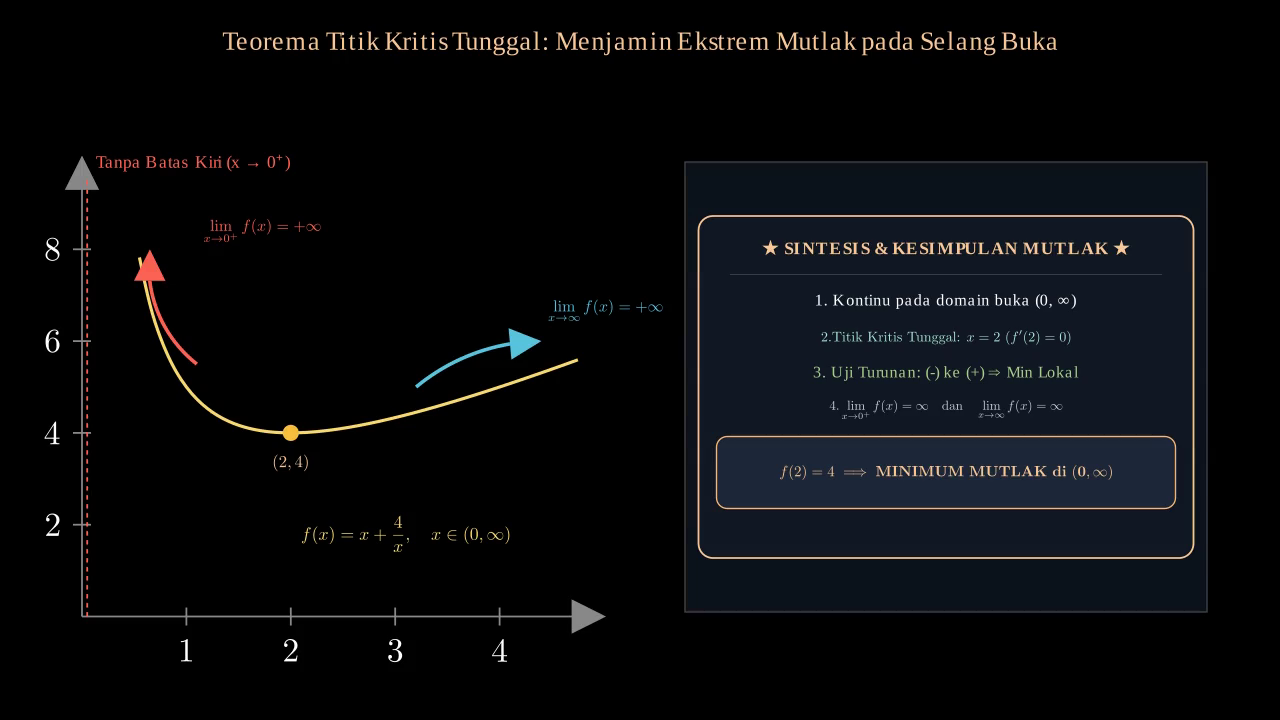
\includegraphics[width=0.92\textwidth]{keyframe_ekstrim_lokal.png}\\
            \vspace{0.05cm}
            {\scriptsize \color{SoftGray} \textit{Eksplorasi Kurva pada $(0, \infty)$: Dari Lokal ke Mutlak}}
        \end{column}
    \end{columns}
\end{frame}

% -------------------------------------------------------------
% Slide 3: Definisi Ekstrem Lokal / Relatif
% -------------------------------------------------------------
\begin{frame}{Definisi Formal: Ekstrem Lokal (\textit{Relative Extrema})}
    \begin{columns}[T]
        \begin{column}{0.48\textwidth}
            \begin{block}{Definisi Ekstrem Lokal}
                Misalkan $S$ daerah asal fungsi $f$ dan $c \in S$:
                \begin{itemize}
                    \item $f(c)$ adalah \textbf{Maksimum Lokal} jika ada selang $I = (c-\delta, c+\delta)$ sehingga:
                    \[
                        f(c) \ge f(x), \quad \forall x \in I \cap S
                    \]
                    \item $f(c)$ adalah \textbf{Minimum Lokal} jika ada selang $I = (c-\delta, c+\delta)$ sehingga:
                    \[
                        f(c) \le f(x), \quad \forall x \in I \cap S
                    \]
                \end{itemize}
            \end{block}
        \end{column}

        \begin{column}{0.48\textwidth}
            \begin{exampleblock}{Intisari Geometris}
                \begin{itemize}
                    \item \textbf{Sifat Topologis}: Hanya meninjau perilaku kurva di sekitar titik $c$ (radius $\delta > 0$).
                    \item \textit{"Raja di desa sendiri"}: Tidak harus terbesar/terkecil pada seluruh semesta $S$.
                    \item Fungsi dapat memiliki \textbf{banyak} puncak \& lembah lokal sekaligus.
                \end{itemize}
            \end{exampleblock}

            \begin{alertblock}{Ekstrem Lokal vs Ekstrem Mutlak}
                Setiap ekstrem mutlak di interior \textbf{pasti} ekstrem lokal, tetapi kebalikannya \textbf{belum tentu} berlaku!
            \end{alertblock}
        \end{column}
    \end{columns}
\end{frame}

% -------------------------------------------------------------
% Slide 4: Di Mana Ekstrem Lokal Dapat Terjadi?
% -------------------------------------------------------------
\begin{frame}{Teorema Titik Kritis Interior: Calon Ekstrem Lokal}
    \begin{block}{Teorema Titik Kritis untuk Ekstrem Lokal (Fermat)}
        Jika fungsi $f$ mencapai nilai ekstrem lokal di titik $c$, maka $c$ \textbf{harus berupa titik kritis interior}, yaitu salah satu dari dua kemungkinan berikut:
    \end{block}

    \vspace{0.06cm}
    \begin{columns}[T]
        \begin{column}{0.48\textwidth}
            \begin{exampleblock}{1. Titik Stasioner}
                Titik di mana turunan bernilai nol:
                \[
                    \mathbf{f'(c) = 0}
                \]
                \begin{itemize}
                    \item Garis singgung berposisi \textbf{mendatar horizontal}.
                    \item Puncak bukit mulus atau dasar lembah bundar.
                \end{itemize}
            \end{exampleblock}
        \end{column}

        \begin{column}{0.48\textwidth}
            \begin{alertblock}{2. Titik Singular}
                Titik di mana turunan \textbf{tidak ada}:
                \[
                    \mathbf{f'(c)\ \text{tidak terdefinisi}}
                \]
                \begin{itemize}
                    \item Sudut tajam (\textit{cusp} / pojok), misal $|x|$ di $x=0$.
                    \item Garis singgung vertikal, misal $x^{2/3}$ di $x=0$.
                \end{itemize}
            \end{alertblock}
        \end{column}
    \end{columns}

    \vspace{0.08cm}
    \centering
    {\scriptsize \color{CoralRose} \textbf{Peringatan Penting}: \textit{Pada selang buka tidak ada titik ujung.}}
\end{frame}

% -------------------------------------------------------------
% Slide 5: Uji Turunan Pertama untuk Ekstrem Lokal
% -------------------------------------------------------------
\begin{frame}{Uji Turunan Pertama (\textit{First Derivative Test})}
    \begin{block}{Teorema Uji Turunan Pertama}
        Misalkan $c$ adalah titik kritis dari fungsi kontinu $f$ pada selang buka yang memuat $c$:
    \end{block}

    \vspace{-0.05cm}
    \begin{columns}[T]
        \begin{column}{0.32\textwidth}
            \begin{alertblock}{1. Maksimum Lokal}
                Tanda $f'$ berubah dari \textbf{$+$ ke $-$}:
                \[
                    f'(x) > 0 \;\xrightarrow{c}\; f'(x) < 0
                \]
                {\scriptsize Menanjak lalu turun $\implies$ terbentuk \textbf{puncak bukit}.}
            \end{alertblock}
        \end{column}

        \begin{column}{0.32\textwidth}
            \begin{exampleblock}{2. Minimum Lokal}
                Tanda $f'$ berubah dari \textbf{$-$ ke $+$}:
                \[
                    f'(x) < 0 \;\xrightarrow{c}\; f'(x) > 0
                \]
                {\scriptsize Meluncur lalu naik $\implies$ terbentuk \textbf{dasar lembah}.}
            \end{exampleblock}
        \end{column}

        \begin{column}{0.32\textwidth}
            \begin{block}{3. Bukan Ekstrem}
                Tanda $f'$ \textbf{tidak berubah}:
                \[
                    +\to +\quad\text{atau}\quad -\to -
                \]
                {\scriptsize Contoh: $f(x) = x^3$ di $x=0$, terus menanjak $\implies$ titik pelana.}
            \end{block}
        \end{column}
    \end{columns}

    \vspace{-0.12cm}
    \begin{exampleblock}{Diagram Garis Bilangan: Kriteria Perubahan Tanda $f'(x)$}
        \centering
        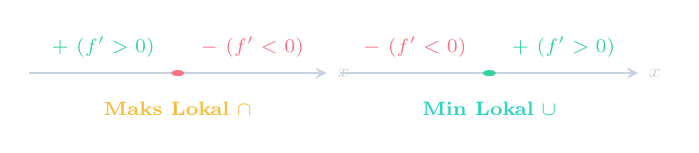
\begin{tikzpicture}[xscale=0.86, yscale=0.35, font=\scriptsize]
            % Kasus Maks: + ke -
            \draw[->, >=stealth, thick, SoftGray] (-2.2, 0) -- (2.2, 0) node[right, SoftGray] {$x$};
            \filldraw[CoralRose] (0, 0) circle (2.5pt) node[below=2pt, white] {$c$};
            \node[above=2pt, EmeraldGreen] at (-1.1, 0) {$\mathbf{+}\ (f' > 0)$};
            \node[above=2pt, CoralRose] at (1.1, 0) {$\mathbf{-}\ (f' < 0)$};
            \node[below=7pt, LuminousGold] at (0, 0) {\textbf{Maks Lokal} $\cap$};

            % Kasus Min: - ke +
            \begin{scope}[shift={(4.6, 0)}]
                \draw[->, >=stealth, thick, SoftGray] (-2.2, 0) -- (2.2, 0) node[right, SoftGray] {$x$};
                \filldraw[EmeraldGreen] (0, 0) circle (2.5pt) node[below=2pt, white] {$c$};
                \node[above=2pt, CoralRose] at (-1.1, 0) {$\mathbf{-}\ (f' < 0)$};
                \node[above=2pt, EmeraldGreen] at (1.1, 0) {$\mathbf{+}\ (f' > 0)$};
                \node[below=7pt, TealCyan] at (0, 0) {\textbf{Min Lokal} $\cup$};
            \end{scope}
        \end{tikzpicture}
    \end{exampleblock}
\end{frame}

% -------------------------------------------------------------
% Slide 6: Uji Turunan Kedua untuk Ekstrem Lokal
% -------------------------------------------------------------
\begin{frame}{Uji Turunan Kedua (\textit{Second Derivative Test})}
    \begin{block}{Teorema Uji Turunan Kedua}
        Misalkan $f'(c) = 0$ dan $f''$ ada pada selang buka yang memuat titik stasioner $c$:
    \end{block}

    \vspace{0.06cm}
    \begin{columns}[T]
        \begin{column}{0.48\textwidth}
            \begin{alertblock}{1. $\mathbf{f''(c) < 0}$ (Cekung ke Bawah $\cap$)}
                \begin{itemize}
                    \item Garis singgung mendatar di puncak mangkok.
                    \item Gradien $f'$ berkurang ($+ \to 0 \to -$).
                    \item $\implies f(c)$ adalah \textbf{Maksimum Lokal}.
                \end{itemize}
            \end{alertblock}
        \end{column}

        \begin{column}{0.48\textwidth}
            \begin{exampleblock}{2. $\mathbf{f''(c) > 0}$ (Cekung ke Atas $\cup$)}
                \begin{itemize}
                    \item Garis singgung mendatar di dasar mangkok.
                    \item Gradien $f'$ bertambah ($- \to 0 \to +$).
                    \item $\implies f(c)$ adalah \textbf{Minimum Lokal}.
                \end{itemize}
            \end{exampleblock}
        \end{column}
    \end{columns}

    \vspace{0.06cm}
    \begin{block}{Kapan Menggunakan Uji I vs Uji II?}
        \begin{itemize}
            \item \textbf{Uji I}: Berlaku untuk semua titik kritis (stasioner \& singular).
            \item \textbf{Uji II}: Cepat jika $f''$ mudah dihitung; inkonklusif jika $f''(c) = 0$.
        \end{itemize}
    \end{block}
\end{frame}

% -------------------------------------------------------------
% Slide 7: Kasus Inkonklusif Uji Turunan Kedua
% -------------------------------------------------------------
\begin{frame}{Jebakan Konseptual: Mengapa Uji Turunan II Gagal Jika $f''(c) = 0$?}
    \begin{alertblock}{Peringatan: Kasus $f'(c) = 0$ dan $f''(c) = 0$}
        Jika $f''(c) = 0$, Uji Turunan Kedua \textbf{inkonklusif}. Nilai $f(c)$ bisa berupa maksimum lokal, minimum lokal, atau bukan ekstrem!
    \end{alertblock}

    \vspace{0.06cm}
    \begin{columns}[T]
        \begin{column}{0.32\textwidth}
            \begin{exampleblock}{Kasus A: $f(x) = x^4$}
                $f'(0)=0,\ f''(0)=0$.\\
                \vspace{0.04cm}
                {\scriptsize Uji I: $f'$ berubah dari $-$ ke $+$.}\\
                \vspace{0.04cm}
                $\implies \mathbf{Min\ Lokal}$!
            \end{exampleblock}
        \end{column}

        \begin{column}{0.32\textwidth}
            \begin{alertblock}{Kasus B: $g(x) = -x^4$}
                $g'(0)=0,\ g''(0)=0$.\\
                \vspace{0.04cm}
                {\scriptsize Uji I: $g'$ berubah dari $+$ ke $-$.}\\
                \vspace{0.04cm}
                $\implies \mathbf{Maks\ Lokal}$!
            \end{alertblock}
        \end{column}

        \begin{column}{0.32\textwidth}
            \begin{block}{Kasus C: $h(x) = x^3$}
                $h'(0)=0,\ h''(0)=0$.\\
                \vspace{0.04cm}
                {\scriptsize Uji I: $h'$ tetap bertanda $+$.}\\
                \vspace{0.04cm}
                $\implies \mathbf{Bukan\ Ekstrem}$!
            \end{block}
        \end{column}
    \end{columns}

    \vspace{0.08cm}
    \centering
    {\small \color{LuminousGold} \textbf{Kaidah Emas}: Jika $f''(c) = 0$, selalu gunakan \textbf{Uji Turunan Pertama}!}
\end{frame}

% -------------------------------------------------------------
% Slide 8: Simulasi Video Interaktif
% -------------------------------------------------------------
\begin{frame}{Simulasi Dinamis: Pelacakan Gradien \& Transisi ke Selang Buka}
    \centering
    % Embedded video untuk presenter (Pympress / PDFPC / Okular)
    \movie[width=8.0cm,height=4.5cm,poster,showcontrols=true]{%
        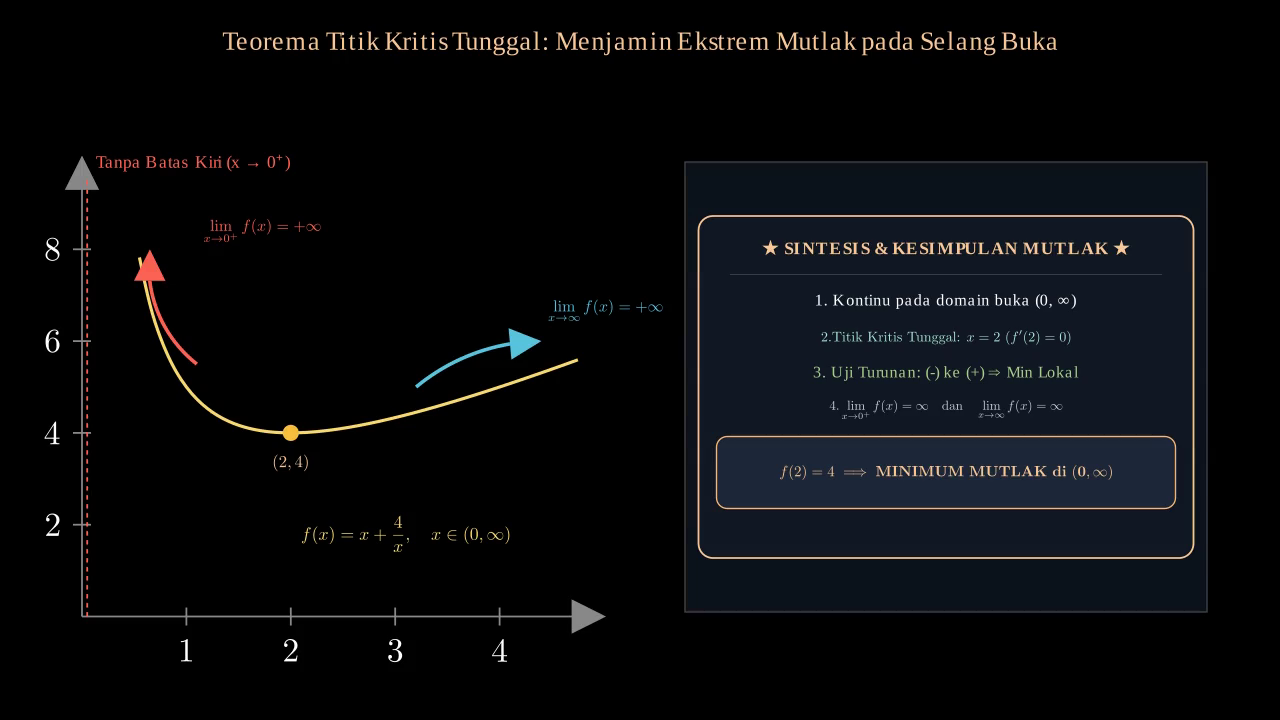
\includegraphics[height=0.48\textheight]{keyframe_ekstrim_lokal.png}%
    }{LocalExtremaOpenIntervalScene.ogv}
    
    \vspace{0.15cm}
    \href{file:LocalExtremaOpenIntervalScene.mp4}{%
        \beamergotobutton{\normalsize $\blacktriangleright$ Putar Video (\texttt{LocalExtremaOpenIntervalScene.mp4})}%
    }
    
    \vspace{0.12cm}
    {\scriptsize \color{SoftGray} \textit{Klik poster untuk pemutaran otomatis di Pympress/Okular, atau klik tombol untuk memutar di MPV/VLC.}}
\end{frame}

% -------------------------------------------------------------
% Slide 9: Ekstrem pada Selang Buka: Mengapa EVT Gagal?
% -------------------------------------------------------------
\begin{frame}{Ekstrem pada Selang Buka: Mengapa EVT Tidak Berlaku?}
    \begin{block}{Kelemahan Domain Terbuka / Tak Terbatas}
        Pada selang buka $(a, b)$ atau selang tak hingga $(0, \infty)$, eksistensi nilai ekstrem mutlak \textbf{tidak lagi dijamin} oleh EVT!
    \end{block}

    \vspace{0.06cm}
    \begin{columns}[T]
        \begin{column}{0.48\textwidth}
            \begin{alertblock}{Skenario 1: Ujung Tak Tercapai}
                $f(x) = x$ pada selang buka $(0, 1)$:
                \begin{itemize}
                    \item $\lim_{x \to 0^+} x = 0$ dan $\lim_{x \to 1^-} x = 1$.
                    \item Nilai $0 \notin (0, 1)$ dan $1 \notin (0, 1)$.
                    \item $\implies$ \textbf{Tidak ada} maks/min mutlak!
                \end{itemize}
            \end{alertblock}
        \end{column}

        \begin{column}{0.48\textwidth}
            \begin{alertblock}{Skenario 2: Melesat ke Tak Hingga}
                $g(x) = \frac{1}{x}$ pada selang buka $(0, 1)$:
                \begin{itemize}
                    \item Saat $x \to 0^+$, nilai $g(x) \to +\infty$.
                    \item Saat $x \to 1^-$, nilai $g(x) \to 1$ ($1 \notin (0, 1)$).
                    \item $\implies$ \textbf{Tidak ada} maks/min mutlak!
                \end{itemize}
            \end{alertblock}
        \end{column}
    \end{columns}
\end{frame}

% -------------------------------------------------------------
% Slide 10: Teorema Titik Kritis Tunggal
% -------------------------------------------------------------
\begin{frame}{Senjata Pamungkas: Teorema Titik Kritis Tunggal}
    \begin{block}{Teorema Titik Kritis Tunggal (\textit{Single Critical Point Theorem})}
        Misalkan $f$ kontinu pada selang $I$ (buka, tutup, atau tak terhingga) dan memiliki \textbf{tepat satu titik kritis} $c \in I$:
        \begin{itemize}
            \item Jika $f(c)$ adalah \textbf{minimum lokal} $\implies f(c)$ adalah \textbf{MINIMUM MUTLAK} pada $I$.
            \item Jika $f(c)$ adalah \textbf{maksimum lokal} $\implies f(c)$ adalah \textbf{MAKSIMUM MUTLAK} pada $I$.
        \end{itemize}
    \end{block}

    \vspace{-0.15cm}
    \begin{columns}[T]
        \begin{column}{0.48\textwidth}
            \begin{exampleblock}{Mengapa Teorema Ini Berdaya?}
                \begin{itemize}
                    \item Menjembatani jurang lokal ke mutlak tanpa syarat selang $[a, b]$.
                    \item Fondasi utama optimasi sains/rekayasa pada domain $(0, \infty)$ (dimensi, waktu, biaya).
                \end{itemize}
            \end{exampleblock}
        \end{column}

        \begin{column}{0.48\textwidth}
            \begin{alertblock}{Logika Pembuktian Kontradiksi}
                \begin{itemize}
                    \item Andaikan ada $x_0$ dengan $f(x_0) < f(c)$, kurva \textbf{harus berbalik arah}.
                    \item Berbalik arah menuntut adanya titik puncak kedua ($f'=0$).
                    \item Kontradiksi keunikan titik kritis tunggal!
                \end{itemize}
            \end{alertblock}
        \end{column}
    \end{columns}
\end{frame}

% -------------------------------------------------------------
% Slide 11: Metode Analisis Limit di Batas Selang Buka
% -------------------------------------------------------------
\begin{frame}{Metode Analisis Perilaku Batas Ujung Selang Buka}
    \begin{columns}[T]
        \begin{column}{0.48\textwidth}
            \begin{exampleblock}{Langkah 1: Titik Kritis Interior}
                \begin{enumerate}
                    \item Hitung turunan pertama $f'(x)$.
                    \item Tentukan semua titik stasioner ($f'=0$) dan titik singular di dalam selang buka $I$.
                    \item Evaluasi nilai fungsi $f(c)$ pada masing-masing titik kritis.
                \end{enumerate}
            \end{exampleblock}
        \end{column}

        \begin{column}{0.48\textwidth}
            \begin{exampleblock}{Langkah 2: Limit di Ujung Batas}
                Hitung perilaku kurva saat mendekati batas ujung selang:
                \[
                    L_1 = \lim_{x \to a^+} f(x), \quad L_2 = \lim_{x \to b^-} f(x)
                \]
                {\scriptsize (Gunakan $\lim_{x \to \infty} f(x)$ jika selang tak terbatas).}
            \end{exampleblock}
        \end{column}
    \end{columns}

    \vspace{0.08cm}
    \begin{alertblock}{Kriteria Penarikan Kesimpulan Ekstrem Mutlak}
        \begin{itemize}
            \item Jika $\mathbf{L_1 = +\infty}$ dan $\mathbf{L_2 = +\infty}$, maka nilai terendah di antara titik-titik kritis dijamin merupakan \textbf{Minimum Mutlak}.
            \item Jika $\mathbf{L_1 = -\infty}$ dan $\mathbf{L_2 = -\infty}$, maka nilai tertinggi di antara titik-titik kritis dijamin merupakan \textbf{Maksimum Mutlak}.
        \end{itemize}
    \end{alertblock}
\end{frame}

% -------------------------------------------------------------
% Slide 12: Contoh Soal 1 (Ekstrem Lokal Polinomial Orde 4)
% -------------------------------------------------------------
\begin{frame}{Contoh Soal 1: Ekstrem Lokal Polinomial Orde 4}
    \textbf{Soal}: Tentukan seluruh titik kritis dan tentukan jenis ekstrem lokal dari fungsi $f(x) = x^4 - 4x^3 + 10$ pada $\mathbb{R}$.

    \pause
    \vspace{0.1cm}
    \begin{columns}[T]
        \begin{column}{0.48\textwidth}
            \begin{block}{Langkah 1: Titik Kritis ($f'$)}
                \[
                    f'(x) = 4x^3 - 12x^2 = 4x^2(x - 3)
                \]
                Titik kritis stasioner ($f'=0$):
                \[
                    x = 0 \quad \text{atau} \quad x = 3
                \]
                Nilai fungsi di titik kritis:
                \begin{itemize}
                    \item $f(0) = 0 - 0 + 10 = \mathbf{10}$
                    \item $f(3) = 81 - 4(27) + 10 = 81 - 108 + 10 = \mathbf{-17}$
                \end{itemize}
            \end{block}
        \end{column}

        \begin{column}{0.48\textwidth}
            \begin{exampleblock}{Langkah 2: Uji Turunan I \& II}
                $f''(x) = 12x(x - 2)$.
                \begin{itemize}
                    \item Di $x = 3$:
                    \[
                        f''(3) = 36 > 0 \implies \cup
                    \]
                    $\implies f(3) = \mathbf{-17}$ (Min Lokal).
                    \item Di $x = 0$: $f''(0) = 0$ \color{CoralRose}(Uji II Inkonklusif!)\\
                    {\scriptsize Uji I: $f'$ bertanda $-$ di kiri/kanan $0$ $\implies$ \textbf{Bukan Ekstrem}!}
                \end{itemize}
            \end{exampleblock}
        \end{column}
    \end{columns}
\end{frame}

% -------------------------------------------------------------
% Slide 13: Contoh Soal 2 (Minimasi pada Selang Buka)
% -------------------------------------------------------------
\begin{frame}{Contoh Soal 2: Ekstrem Mutlak pada Selang Buka $(0, \infty)$}
    \textbf{Soal}: Tentukan nilai ekstrem mutlak dari $f(x) = x + \frac{4}{x}$ pada selang buka $(0, \infty)$.

    \pause
    \vspace{0.08cm}
    \begin{columns}[T]
        \begin{column}{0.48\textwidth}
            \begin{block}{Langkah 1: Titik Kritis}
                Turunan pertama:
                \[
                    f'(x) = 1 - \frac{4}{x^2} = \frac{x^2 - 4}{x^2}
                \]
                Syarat stasioner $f'(x) = 0$:
                \[
                    x^2 - 4 = 0 \implies x = \pm 2
                \]
                Karena $x \in (0, \infty) \implies \mathbf{x = 2}$.\\
                Nilai fungsi: $f(2) = 2 + \frac{4}{2} = \mathbf{4}$.
            \end{block}
        \end{column}

        \begin{column}{0.48\textwidth}
            \begin{exampleblock}{Langkah 2: Uji Kritis Tunggal}
                $f''(2) = \frac{8}{2^3} = 1 > 0 \implies \cup$ (\textbf{Min Lokal}).\\
                \vspace{0.05cm}
                Limit di batas $(0, \infty)$:
                \[
                    \lim_{x \to 0^+} f(x) = \infty, \quad \lim_{x \to \infty} f(x) = \infty
                \]
                \textbf{Kritis Tunggal}: Karena $x=2$ adalah satu-satunya titik kritis pada $(0, \infty)$, maka $f(2) = 4$ adalah \textbf{MINIMUM MUTLAK} pada $(0, \infty)$!
            \end{exampleblock}
        \end{column}
    \end{columns}
\end{frame}

% -------------------------------------------------------------
% Slide 14: Aplikasi Pemodelan Terapan
% -------------------------------------------------------------
\begin{frame}{Aplikasi Pemodelan: Desain Kemasan Optimal pada $(0, \infty)$}
    \textbf{Masalah}: Kaleng silinder tertutup bervolume $V = 54\pi\text{ cm}^3$. Tentukan jari-jari $r$ dan tinggi $h$ yang meminimumkan luas permukaan!

    \pause
    \vspace{0.08cm}
    \begin{columns}[T]
        \begin{column}{0.48\textwidth}
            \begin{block}{Pemodelan Matematis}
                Volume: $V = \pi r^2 h = 54\pi \implies h = \frac{54}{r^2}$.\\
                \vspace{0.04cm}
                Luas silinder tertutup:
                \[
                    A(r) = 2\pi r^2 + \frac{108\pi}{r}, \quad r \in (0, \infty)
                \]
                {\scriptsize Domain berupa selang buka $(0, \infty)$.}
            \end{block}
        \end{column}

        \begin{column}{0.48\textwidth}
            \begin{exampleblock}{Optimasi \& Kritis Tunggal}
                Titik stasioner:
                \[
                    A'(r) = 4\pi r - \frac{108\pi}{r^2} = 0 \implies r = 3
                \]
                Uji kelengkungan:
                \[
                    A''(3) = 4\pi + 8\pi = 12\pi > 0 \implies \cup
                \]
                $\implies \mathbf{r = 3\text{ cm}}$ adalah \textbf{Minimum Mutlak}!\\
                Tinggi kaleng: $h = \frac{54}{3^2} = \mathbf{6\text{ cm}}$ ($h = 2r$).
            \end{exampleblock}
        \end{column}
    \end{columns}
\end{frame}

% -------------------------------------------------------------
% Slide 15: Latihan Mandiri & Rangkuman Kaidah
% -------------------------------------------------------------
\begin{frame}{Latihan Mandiri \& Rangkuman Subtopik 3.3}
    \begin{columns}[T]
        \begin{column}{0.48\textwidth}
            \begin{block}{Latihan Mandiri Persiapan UTS}
                \begin{enumerate}
                    \item Titik kritis dan jenis ekstrem:
                    \[
                        f(x) = x^{2/3}(5 - x)
                    \]
                    \item Nilai minimum mutlak biaya rata-rata pada $q \in (0, \infty)$:
                    \[
                        C(q) = \frac{50}{q} + 2q + 8
                    \]
                \end{enumerate}
            \end{block}
        \end{column}

        \begin{column}{0.48\textwidth}
            \begin{exampleblock}{Rangkuman Kaidah Ekstrem}
                \centering
                \scriptsize
                \setlength{\tabcolsep}{1.5pt}
                \begin{tabular}{|l|l|}
                    \hline
                    \textbf{Domain} & \textbf{Strategi Penentuan} \\
                    \hline
                    Tertutup $[a, b]$ & Metode Selang Tertutup \\
                    Lokal & Uji Turunan I / II \\
                    Kritis Tunggal & Lokal $\implies$ Mutlak! \\
                    Buka $(a, b)$ & Analisis Limit Ujung \\
                    \hline
                \end{tabular}
            \end{exampleblock}

            \vspace{0.12cm}
            \centering
            {\small \textbf{Selamat Belajar \& Sukses MA1101!}}\\
            {\scriptsize \color{SoftGray} Tim Dosen Matematika I --- FMIPA ITB}
        \end{column}
    \end{columns}
\end{frame}

\end{document}
